\documentclass[notitlepage,letterpaper, 10pt]{article}
\usepackage[ansinew]{inputenc} % Acepta caracteres en castellano
\usepackage[colorlinks=true,urlcolor=blue,linkcolor=blue,citecolor=blue]{hyperref} % navega por el doc
\usepackage{amsmath}
\usepackage{amsfonts}
\usepackage{amssymb}
\usepackage{graphicx}
\usepackage{subfig}
\usepackage{cancel}
\usepackage{booktabs}
\usepackage{color}
%\usepackage{geometry}      % See geometry.pdf to learn the layout options.
%\geometry{letterpaper}                   % ... or a4paper or a5paper or ... 
%\usepackage{epstopdf}
%\usepackage{subfigure} 
%\usepackage{iopams}  

%\usepackage{amsmath}

\usepackage{amsthm}
\usepackage{lineno}
\linenumbers


\begin{document}

\title {Matching Conditions\\ for Radiation Hydrodynamics \\ in General Relativistic Spheres}
\author{
L.F. Casta\~neda-Godoy\thanks{fabian2121015@gmail.com} \\
\textit{Escuela de F\'isica, Universidad Industrial de Santander,}\\ \textit{Bucaramanga-Colombia} \, ; \\
L.A. N\'u\~nez\thanks{lnunez@uis.edu.co} \\
\textit{Escuela de F\'isica, Universidad Industrial de Santander,}\\ \textit{Bucaramanga-Colombia} \\ 
\textit{and Departamento de F\'isica, Universidad de Los Andes,}\\ \textit{M\'erida-Venezuela} \\
and J. Ospino\thanks{j.ospino@usal.es}, \\ \textit{Departamento de Matem\'atica Aplicada and} \\
\textit{Instituto Universitario de F\'isica Fundamental y Matem\'aticas,}  \\ \textit{ Universidad de Salamanca, Salamanca-Spain;} \\
}
\maketitle

\begin{abstract}
By applying a 
\end{abstract} 
PACS: 04.40.-b, 04.40.Nr, 04.40.Dg \\
Keywords: Relativistic Fluids,spherical  and non-spherical sources, interior solutions.
\maketitle

\section{Introduction}

Conscious of the difficulties to cope with dissipation due to the emission of photons and/or neutrinos in ultradense matter --and, aware of the uncertainties of the microphysics when considering the interaction between radiation and matter at these densities-- we introduce a relation between the radiation energy flux density and the radiation energy density, i.e. the \textit{flux factor,} $f = {\mathcal{F}}/{\rho_{R}},$ and the so-called \textit{variable Eddington factor,} $\chi= {\mathcal{P}}/{\rho_{R}}, $ relating the radiation pressure and the radiation energy density. We have also included a closure relation between both quantities, i.e., $\chi=\chi(f).$ In the literature, several closures have been introduced (see references \cite{Levermore1984, Dominguez1997, PonsIbanezMiralles2000, SmitVandenHornBludman2000} and particularly \cite{MurchikovaAbdikamalovUrbatsch2017} for more recent and complete study) and most of them are consistent with the hyperbolicity and causality required by a relativistic theory \cite{PonsIbanezMiralles2000}.


\section{Radiating Spheres}
\subsection{Metric and Einstein Equations}
\label{GeneralEquations}
Let us consider a spherically symmetric  space-time whose line element is given by
\begin{equation}
ds^2= e^{2\nu(r,t)}\mathrm{d}t^2-e^{2\lambda(r,t)} \mathrm{d}r^2-r^2(\mathrm{d}\theta^2 + \sin^{2}\theta \mathrm{d}\phi^2), \label{metric}    
\end{equation}
and its corresponding Einstein equations, $-G^\nu_\mu = 8\pi T^\nu_\mu$, written as:
\begin{align}
8\pi T^0_0 &=\frac{1}{r^2} -e^{-2\lambda}\left(\frac{1}{r^2}-\frac{2\lambda'}{r} \right),
\label{EinsEq00} \\
8\pi T^1_1 &= \frac{1}{r^2} -e^{-2\lambda} \left(\frac{1}{r^2}+\frac{2\nu'}{r}\right),
\label{EinsEq11} \\
8\pi T^2_2 &= 8\pi T^3_3 = e^{-2\lambda} \left(\nu^{\prime \prime}+(\nu^{\prime})^2 -\lambda^{\prime}\nu^{\prime} + \frac{\nu^{\prime} - \lambda^{\prime}}{r}\right)
-e^{-2\nu}\left(\ddot{\lambda} +\dot{\lambda}(\dot{\lambda}-\dot{\nu})\right)
\label{EinsEq22} \\
8\pi T_{01} &=\frac{2\dot\lambda}{r},
\label{EinsEq01}
\end{align}
where dots and primes represent derivatives with respect to $t$ and $r$, respectively.

Let us assume that the energy momentum tensor can be split in two constituents, $T_{\mu\nu} = T_{\mu\nu}^{M} + T_{\mu\nu}^{R}$, where $T_{\mu\nu}^{M}$ stands for the  material part while $T_{\mu\nu}^{R}$ represents the radiation contribution, and can be written as:
\begin{equation}
\label{TmunuMat}
{T}^{M}_{\mu \nu}= (\rho + P_{\perp}) u_\mu u_\nu - P_{\perp} g_{\mu \nu}  + (P-P_{\perp}) v_\mu v_\nu  ,
\end{equation}
and 
\begin{equation}
\label{TmunuRad}
T^{R}_{\mu \nu}= \frac{1}{2}(3\rho_{R}-\mathcal{P})u_\mu u_\nu - \frac{1}{2}(\rho_{R}-\mathcal{P})g_{\mu \nu}  +\frac{1}{2}(\rho_{R} -3\mathcal{P})v_\mu v_\nu  + F_\mu u_\nu + F_\nu u_\mu \,,
\end{equation}
with 
\begin{equation}
u_\mu = \gamma (\mathrm{e}^{\nu}, -\omega \mathrm{e}^{\lambda}, 0, 0) , \;
v_\mu = \gamma (-\omega \mathrm{e}^{\nu}, \mathrm{e}^{\lambda}, 0, 0)  \; \mathrm{and} \;
F_\mu =  \mathcal{F}v_\mu. 
\label{umu}
\end{equation}
where the Lorentz factor is $\gamma=\left(1-\omega^2 \right)^{-\frac{1}{2}}$ and the fluid velocity is defined as
\begin{equation}
\omega = \frac{\mathrm{d} r}{ \mathrm{d} t} \mathrm{e}^{\lambda -\nu}
\label{velocity1}
\end{equation}
The matter physical variables --as measured by a com-moving minkowskian observer--  are the energy density, $\rho$; radial pressure $P$ and tangential pressure $P_{\perp}$.  The corresponding radiation variables --also evaluated at the local com-moving rest frame-- are radiation energy density $\rho_{R}$, radiation energy flux, $\mathcal{F}$, and radiation pressure $\mathcal{P}$. These variables, for spherical symmetry case, can be written  in terms of the specific intensity $\mathbf{I}(r,t;\vec{n},\nu)$ as \cite{Lindquist1966,MihalasMihalas1984,RezzollaMiller1994}:
\begin{equation}
\rho_{R}=\frac{1}{2} \int_{0}^{\infty}d\nu  \int_{1}^{-1}d\mu \, \mathbf{I}(r,t;\vec{n},\nu), \quad \mathcal{F}=\frac{1}{2} \int_{0}^{\infty}d\nu  \int_{1}^{-1}d\mu \, \mu  \mathbf{I} (r,t;\vec{n},\nu)\label{eq_0mom} 
\end{equation}
and
\begin{equation}
\mathcal{P}=\frac{1}{2} \int_{0}^{\infty}d\nu\hspace{0.25cm}\int_{1}^{-1}
d\mu\, \mu^{2} \, \mathbf{I}(r,t;\vec{n},\nu) \,.\label{eq_2mom}
\end{equation}
where
\begin{equation}
\mathrm{d}\mathcal{E}=\mathbf{I}(r,t;{\vec{n}},{\nu})\mathrm{d}S\ \cos
\varphi\ \mathrm{d}\Theta\ \mathrm{d}\upsilon\ \mathrm{d}t,
\end{equation}
$\mathrm{d}\mathcal{E}$ is defined as the energy transported by a radiation of frequencies $\left(  \nu,\nu +\mathrm{d}\nu \right)$ in time $\mathrm{d}t,$ crossing a surface element $\mathrm{d}S,$ through the solid angle around ${\vec{n},}$ i.e. $\mathrm{d}\Theta \equiv
 \sin\theta \, \mathrm{d}\theta \, \mathrm{d}\psi \equiv -\mathrm{d}\mu \, \mathrm{d}\psi$, with $\varphi$ the angle between ${\vec{n}}$ and the normal to $\mathrm{d}S$.
 
Clearly in the language of radiation-hydrodynamics, equations (\ref{eq_0mom}) and (\ref{eq_2mom}) represent the moments of the radiation field $\mathbf{I}(r,t;\vec{n},\nu)$, which describes the physical properties of the medium (absorption and emission). The zero-moment is the radiation energy density, $\rho_{R}$, the first-moment the energy flux density, $\mathcal{F}$ and the second-moment the radiation pressure $\mathcal{P}$.    

The above, Einstein equations (\ref{EinsEq11})-(\ref{EinsEq01}) can also be re-written regarding the physical variables as
\begin{align}
    8\pi \left( \frac{\bar{\rho}+ \omega^2 \bar{P} +2 \omega {\cal F}}{1-\omega^2} \right) & =  
    \frac{1}{r^2} -e^{-2\lambda}\left(\frac{1}{r^2}-\frac{2\lambda'}{r} \right) \, , \label{EinsEq200} \\
    8\pi \left( \frac{\bar{P}+\omega^2 \bar{\rho} + 2 \omega {\cal F}}{1-\omega^2} \right) & 
    = \frac{1}{r^2} -e^{-2\lambda} \left(\frac{1}{r^2}+\frac{2\nu'}{r}\right)\, , \label{EinsEq211} \\
8\pi \bar{P}_{\perp}& =  e^{-2\lambda} \left(\nu^{\prime \prime}+(\nu^{\prime})^2 -\lambda^{\prime}\nu^{\prime} + \frac{\nu^{\prime} - \lambda^{\prime}}{r}\right) 
\nonumber \\
& \qquad - e^{-2\nu}\left(\ddot{\lambda} +\dot{\lambda}(\dot{\lambda}-\dot{\nu})\right) \, , \label{EinsEq222} \\   
8\pi e^{\frac{\nu+\lambda}{2}}\left(\frac{ \omega(\bar{\rho}+\bar{P})+(1+\omega^2){\cal F}}{1-\omega^2} \right)& = -\frac{\dot{\lambda}}{r}\, , \label{EinsEq201}
\end{align}
where we have also used several intermediate variables:
\begin{equation}
\bar{\rho}=\rho+ \rho_{R} \,, \;
\bar{P}= P+ \mathcal{P} \,, \; 
\bar{P}_{\perp}= P_{\perp}+ \mathcal{P}_{\perp} \; \textrm{and} \;
\mathcal{P}_{\perp}=\frac{\rho_{R}-\mathcal{P}}{2} . 
\end{equation}
Now by using the post-quasi-static ``effective'' density and pressure,  \cite{HerreraEtal2002,NunezRueda2007,NavarroEtal2008}:
 \begin{equation}
\tilde{\rho} =\frac{\bar{\rho} + \bar{P}\omega^{2}+ 2 \mathcal{F}\omega}{1-\omega^{2}},
 \qquad
\tilde{P} = \frac{\bar{\rho} \omega^{2}+\bar{P}+ 2 \mathcal{F}\omega}{1-\omega^{2}} ,
\label{VariableEf2}
 \end{equation}
we can re-shape the above field equations as:
\begin{align}
m^{\prime } &= 4 \pi r^{2}\tilde{\rho}, \label{EinsEq300}  \\
\nu^{\prime} & = \frac{4\pi r^{3}\tilde{P}+ m}{r(r-2m)}, \label{EinsEq311} \\
8\pi \bar{P}_{\perp} &= \left\{ \left( 1-\frac{2m}{r} \right) \left( \nu^{\prime \prime} + (\nu^{\prime})^{2}+ \frac{\nu^{\prime}}{r}  \right) + \left(  \frac{m}{r^{2}} -\frac{m^{\prime }}{r}  \right) \left( \nu^{\prime} + \frac{1}{r}     \right)   \right\} 
\nonumber \\ 
& \qquad  + \frac{e^{-2\nu}}{4} \left\{ 2\left(1 - \frac{2m}{r} \right)^{-1}
\left( \frac{\ddot{m}}{r} +\frac{2\dot{m}^2}{r^2} \left(1 - \frac{2m}{r} \right)^{-1}
\right)\right. \nonumber \\
& \qquad + \left.
\frac{\dot{m}}{r}\left(1 - \frac{2m}{r} \right)^{-1}
\left(\frac{\dot{m}}{r}\left(1 - \frac{2m}{r} \right)^{-1} -\dot{\nu}
\right)
\right\} \; \textrm{and} \label{EinsEq322} \\
\dot{m} &= -\frac{4 \pi r^{2} e^{\nu-\lambda}}{1+\omega^{2}}\left( \omega(\tilde{\rho}+ \tilde{P})+ (1-\omega^{2})\mathcal{F}     \right)  \label{EinsEq301}\, ;
\end{align}
with the metric function $\lambda(r,t)$ expressed in terms of the Misner ``mass function'' as \cite{HernandezMisner1966}
\begin{equation}
 m(t,r)=\frac{r^2}{2}R^{3}_{232} \; \Leftrightarrow \; m(r,t)=4\pi \int ^r_0 T^0_0r^2\mathrm{d}r \; \Rightarrow e^{-2\lambda}= 1-\frac{2 m(r,t)}{r}.
\label{MassDef} 
 \end{equation}
 
\subsection{Quasi-static evolution framework}
In this section, we shall describe the Quasi-static evolution framework. In this approximation, we neglect terms in second-order time-derivatives, quadratic in time-derivatives and quadratic in radial velocity, i.e.
\begin{equation}
\label{QSassumption}
\omega^{2} \approx 
\ddot{\lambda}\approx\dot{\lambda}^2\approx\dot{\lambda}\dot{\nu}\approx\ddot{\nu}\approx 0 \, .
\end{equation}
From (\ref{EinsEq200})-(\ref{EinsEq201}), we can obtain
\begin{equation}\label{hydrostatic}
\ddot{\lambda}+{\dot{\lambda}^2}-{\dot{\lambda} \dot{\nu} }=4\pi r{\rm e}^{2\nu}\left(\bar{P}^{\prime}+{(\bar{\rho} +\bar{P})\nu^{\prime}}-\frac{2(\bar{P}_\perp -\bar{P})}{r}\right)  
\end{equation}
which, under the quasi-static assumptions (\ref{QSassumption}), leads to the hydrostatic equilibrium equation, 
\begin{equation}\label{TOVanisotropic}
\bar{P}^{\prime}+{(\bar{\rho} +\bar{P})\nu^{\prime}}-\frac{2(\bar{P}_\perp -\bar{P})}{r}= 0 \; .
\end{equation} 
Thus, if the radial velocity, $\omega$, as well as its radial and time derivatives, are considered small and their products neglected, the system evolves through a series of hydro-static equilibrium phases  -in a time scale that is very long compared to the typical hydro-static time.  Moreover, from equation (\ref{EinsEq201}) it can be appreciated that the energy flux density ${\cal F}$ is of the order $\omega$ within the quasi-static approximation\cite{HerreraDiPrisco1997,BecerraHernandezNunez2015}.
It is worth to be noticed that this approach is self-consistent, i.e., if you accept that equation (\ref{TOVanisotropic}) is always satisfied during the evolution the physical variables, then the assumptions (\ref{QSassumption}) will be recovered.

When the quasi-static approximation is considered the effective variables (\ref{VariableEf2}) becomes $\tilde{\rho} \approx \bar{\rho}= \rho+ \rho_{R}$ and $\tilde{P} \approx \bar{P} = P+ \mathcal{P}$, and the system (\ref{EinsEq300})-(\ref{EinsEq301}) can be re-written as
\begin{align}
m^{\prime} &= 4 \pi r^{2}\tilde{\rho}, \label{EinsEq400} \\
\nu^{\prime} & = \frac{4\pi r^{3}\tilde{P}+ m}{r(r-2m)}, \label{EinsEq411} \\
8\pi \bar{P}_{\perp} &= \left\{ \left( 1-\frac{2m}{r} \right) \left( \nu^{\prime \prime} + (\nu^{\prime})^{2}+ \frac{\nu^{\prime}}{r}  \right) + \left(  \frac{m}{r^{2}} -\frac{m^{\prime }}{r}  \right) \left( \nu^{\prime} + \frac{1}{r}     \right)   \right\} \, ,  \label{EinsEq422} \\
\; \textrm{and} \quad \dot{m} &= 
-\dfrac{4 \pi r^{2}}{1+\omega^{2}} e^{\nu-\lambda}
\left( \omega(\bar{\rho}+ \bar{P})+ \mathcal{F}\left( 1-\omega^{2}\right) \right)  \label{EinsEq401}\, .
\end{align}


\subsection{Eddington factors and the radiation field}
It is clear that to deal with more realistic astrophysical scenarios, a relativistic Boltzmann Transport Equation should be considered to describe the evolution of the radiation through the matter configuration\cite{Lindquist1966}.  Despite this, it is possible to find several other physically interesting situations correspondint to two limits approximation for the radiation field, namely, {\em free streaming out} and {\em diffusion} \cite{MihalasMihalas1984}. 

The {\em free streaming out} limit assumes that radiation (neutrinos and, or, photons) mean free path is of the order of the dimension of the sphere. With this assumption, we obtain
\begin{equation}
\rho_{R} = {\cal F} = {\cal P} = \hat{\epsilon} \; .  \label{free_streaming}
\end{equation}
On the other hand, in the {\em diffusion limit approximation} radiation is considered to flow within distances much smaller than the characteristic length of the system. Within this limit, radiation is locally isotropic, and we have 
\begin{equation}
\rho_{R} = 3 {\cal P} \hspace{.5cm} and \hspace{.5cm} {\cal F} = {\hat{q}}
\; .  \label{diffusio_appox}
\end{equation}

We implement the flux, $f$, and the variable Eddington factor, $\chi$ to describe radiation-hydrodynamic scenarios between the above mentioned two limits. Let us consider equations (\ref{eq_0mom}) through (\ref{eq_2mom}) and define the following normalized quantities 
\begin{equation}
\varphi(\vec{r},t,\Omega) = \frac{I(\vec{r},t, \Omega)}{\rho_{R}}, \quad \mathbf{\vec{f}}=\int_{4\pi}\varphi(\vec{r},t,\Omega)\vec{n}\, d\Omega   \label{normalizequantities1}%
\end{equation}
and
\begin{equation}
 \mathbb{K}=\int_{4\pi}\varphi(\vec{r},t,\Omega)\vec{n}\otimes\vec{n}\,d\Omega, \label{normalizequantities2}%
\end{equation}
Now, the Eddington factor can be defined as the eigenvalue of the Pressure Tensor corresponding to the eigenvector $\vec{n}$ (unitary vector in the direction of the energy flux ), i.e. $K_{j}^{i}n^{j}=\chi n^{i}$ \cite{AnilePennisiSammartino1991}. Thus,
\begin{equation}
\mathbf{\vec{f}} \Rightarrow f^{i}=fn^{i} \quad \text{and} \quad \mathbb{K\Rightarrow} K^{ij} = 
\frac{1}{2}\left\{  (1-\chi)\delta^{ij}+(3\chi-1)n^{i}n^{j}\right\}. \label{EddingtonAnile1}%
\end{equation}
In the one-dimensional spherical case the above equations lead to%
\begin{equation}
f=\frac{\mathcal{F}}{\rho_{R}\text{ }}\mathrm{\quad}\text{and}\mathrm{\quad
}\mathcal{\chi}=\frac{\mathcal{P}}{\rho_{R}}\, . \label{EddingtonAnile2}%
\end{equation}

%voy por aquí

\subsection{Closures relations}
In order to ``close'' this problem and to algebraically obtain six of the above mentioned physical variables --namely $\omega$, $\rho$, $\rho_R$, $P$, $P_{\perp}$ $\mathcal{P}$ and $\mathcal{F}$-- from field equations (\ref{EinsEq11}) through (\ref{EinsEq01}) and the radiation parameter (\ref{EddingtonAnile2}) (or in general from equations (\ref{normalizequantities1}) and \ref{normalizequantities2})); we need to state a relation between $f$, and $\chi$. It is easy to perceive that such a relation could exist. 

In fact, equations (\ref{diffusio_appox}) and (\ref{free_streaming}) correspond to the most simple closure relations. In the free-streaming out limit --optically thin approximation-- the three moments are forced to be equal, represented a highly anisotropic distribution of radiation pressures.  In the diffusion limit approximation --optically thick limit--, the first moment can be approximated using the gradient of the zeroth moment via the Fick's law, while the second moment is one-third of the zeroth moment\cite{Pomraning1983}. In this case, we have an isotropic radiation field within the matter configuration. 

It is noticeable that for the intermediate cases for the radiation field, we have
\begin{equation}
\left.
\begin{array}
[c]{c}%
\mathcal{P}=\frac{1}{3}\rho_{R} \Rightarrow f \longrightarrow 0 \; \text{and} \; \chi = \frac{1}{3}\\
\\
\mathcal{F}= \mathcal{P=} \rho_{R} \Rightarrow f = 1 \; \text{and} \; \chi=1
\end{array}
\right\}  \Rightarrow 0 \leq f \leq 1 \; \text{and} \; \frac{1}{3} \ \leq \chi(f) \leq 1. \label{efeji}%
\end{equation}
In this case we close the system expressing the second and the third moments in terms of the lower-order moments using simple analytic relations. 

The above closing schema are often called the M1 methods\cite{SmitVandenHornBludman2000,PonsIbanezMiralles2000,SmitCernohorskyDullemond1997A,SmitCernohorskyDullemond1997B} or or the ``algebraic Eddington factor'' methods \cite{JustObergaulingerJanka2015,MurchikovaAbdikamalovUrbatsch2017} and were originally proposed in several seminal works\cite{Levermore1984,Pomraning1969,Kershaw1976}. 


Causality requirement implies the following supplementary conditions on $f$ and $\chi,$ in order to define a physically plausible region in the 
$\left\{ f,\chi, \mathrm{d}\chi/{\mathrm{d}f} \right\}  $ space
\cite{PonsIbanezMiralles2000}%
\begin{equation}
\left\|  f\right\|  \leq 1, \quad f^{2}\leq \chi \leq 1 \quad   \text{and} \quad - \frac{1-\chi}{1+f} \leq \frac{\mathrm{d}\chi}{\mathrm{d}f} \leq \frac{1-\chi}{1-f} \, . \label{condfdxi}%
\end{equation}%

Table \ref{tabla1} lists 7 of the closure relations most frequent found in the literature. In this list the first five could be considered as ``analytical'', they are simply \textit{ad hoc} relations that smoothly interpolate the radiation field between the diffusive and free-streaming regimes\cite{LeblancWilson1970,WilsonEtal1975,Kershaw1976}. Others, are derived from a maximum entropy principle or from a given, or assumed, angular dependence of the radiative distribution functions\cite{Minerbo1978,CernohorskyBludman1994}. Even one of them has been motivated from direct transport Monte Carlo simulations. While the last two are referred as numerical, because for a given flux factor $f,$ the nonlinear equation $f=\coth\beta-({1}/{\beta})$ has to be numerically solved in order to obtain the variable Eddington factor $\chi$\cite{Minerbo1978}.    

\begin{table}[ht] \centering
{\small 
\begin{tabular}
[c]{|c|c|}\hline\hline 
\textbf{Closure} & $\chi(f)  $  \\ \hline\hline
\textit{Kershaw } (Ke) \cite{Kershaw1976}   & $\frac{1 + 2 f^2}{3}$ \\ \hline
\textit{Lorentz-Eddington }(LE)    & $\frac{5}{3}-\frac {2}{3}\sqrt{4-3f^{2}}$ \\\hline
\textit{Bowers-Wilson} (BW) \cite{WilsonEtal1975}  & $\frac{1}{3}\left( 1-f+3f^{2}\right)$ \\ \hline
\textit{Levermore-Lorentz} (LL) \cite{Levermore1984}  & $\frac{3 +4f^2 }{5 +2\sqrt{ 4 -3f^2}}$ \\ \hline
\textit{Janka (Monte Carlo) } (MC)  & $\frac{1}{3}\left( 1+\frac{1}{2}f^{1.31} + \frac{3}{2}f^{4.13} \right)  $ \\ \hline 
\textit{Maximum Packing} (MP)      & $\frac{1}{3}\left( 1-2f+4f^{2}\right)  $ \\ \hline 
\textit{Minerbo} (Mi) \cite{Minerbo1978} & $1 -2\frac{f}{\kappa}$   where $f=\coth\kappa -\frac{1}{\kappa}$ \\\hline
\textit{Levermore-Pomraning} & $f\coth\beta $ where $f= \coth\beta- \frac{1}{\beta}$ \\\hline
\end{tabular}
}
\caption{Closure Relations and some of their physical acceptability conditions}
\label{tabla1}
\end{table}



\section{Surfaces and Matching Conditions}
As we have pointed out above, we are going to express the equations that describe the evolution of different types of surfaces, in general relativistic --spherical and plane-parallel flow-- radiation-hydrodynamic scenarios. 

\begin{figure}[!ht]
\begin{center}
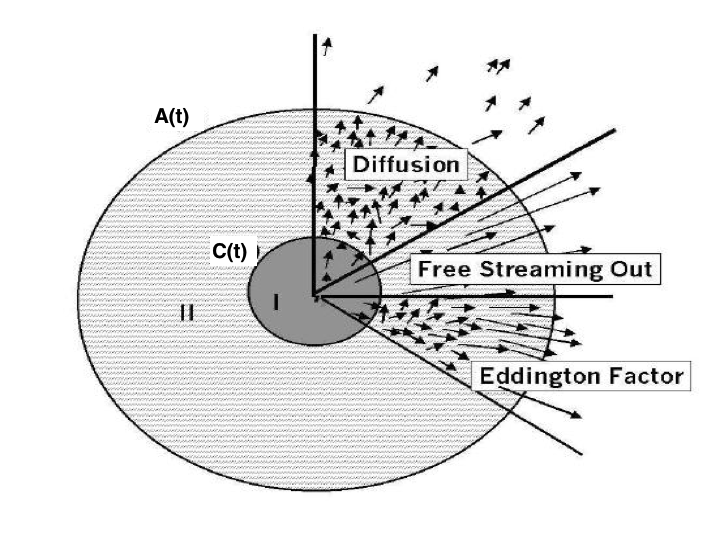
\includegraphics[width=0.6\textwidth]{GridChoqueEsfera.png}
\caption{Regions of the matter distribution. The core is labeled by $I$ is the more compact one; the mantle ($II$) is the region in the middle and the exterior space--time ($III$). The region $I$ and $II$ is separated by discontinuity surface $r = C(t)$, while the matter configurations is delimited by a boundary surface $r =A(t)$. The {\em free streaming out} limit assumes that radiation (neutrinos and, or, photons) mean free path is of the order of the dimension of the sphere. The {\em diffusion limit approximation} radiation is considered to flow within distances much smaller than the characteristic length of the system. We implement the flux, $f$, and the variable Eddington factor, $\chi$ to describe radiation-hydrodynamic scenarios between the above mentioned two limits.}
\label{Sphere}
\end{center}
\end{figure}


In the next section we sketch the matching conditions in terms of the null tetrad Newman-Penronse formalism

\subsection{Matching conditions}
In general relativistic hydrodynamic is of paramount importance to accurately match two solutions of the Einstein equations through --for our case a non-null hypersurface--, which may represent separated regions filled with different fluids and dynamics\cite{BonnorVickers1981}. 

Let us consider a non-null hypersurface $C$ that separates two space-time regions $M$ and $M'$, containing matter and radiation, $T_{\mu\nu} = T_{\mu\nu}^{M} + T_{\mu\nu}^{R}$, described by equations (\ref{TmunuMat}) and (\ref{TmunuRad}).

In 1983 L. Herrera and J. Jim\'enez \cite{HerreraJimenez1983} presented a set of junction conditions, regarding the Newman-Penrose, NP, variables (tetrad vectors and spin coefficients)\cite{NewmanPenrose1962}, equivalent to the standard Darmois\cite{Darmois1927} and Lichnerowicz\cite{Lichnerowicz1955} conditions. Recently, the continuity of the eigenvalues of the Riemann curvature tensor proves to play an important role to express the matching conditions \cite{GutierrezQuevedo2019}.     

The Herrera-Jim\'enez approach has been particularly useful in describing astrophysical scenarios involving some of the above types of discontinuities, mainly mass shells where spin coefficients are discontinuous scalars\cite{HerreraEtal1987, HerreraIbanez1989, EsculpiHerrera1994}. 

Now the metric is described in the complex null tetrad NP formalism as
\begin{equation}
g_{\mu \nu}=  n_{\mu } l_{\nu}+ l_{\mu }n_{\nu} - m_{\mu } \bar{m}_{\nu} - \bar{m}_{\mu }m_{\nu}, 
\label{nulltetrad}
\end{equation}
with the  complex null tetrad satisfies 
$ l_{\mu}n^{\mu}= -m_{\mu} \bar{m}^{\mu}=1 $ and \\
$l_{\mu}l^{\mu}= n_{\mu}n^{\mu}=m^{\mu}m_{\mu }= \bar{m}_{\mu} \bar{m}^{\mu}=l_{\mu}m^{\mu}=l_{\mu}\bar{m}^{\mu}= n_{\mu}m^{\mu}=n_{\mu}\bar{m}^{\mu}=0,$ where the bar indicates the complex conjugate of an object: $m^{\mu} \longrightarrow \bar{m}^{\mu}$.

The spin coefficient are defined from the directional derivatives along the null tetrad  as\cite{NewmanPenrose1962,HerreraJimenez1983}:
\begin{align*}
 D\,n^\mu -\Delta\,l^\mu = &
-(\gamma -\bar{\gamma})l^{\mu} + (\pi + \bar{\tau})m^{\mu} +
(\bar{\pi} + \tau)\bar{m}^{\mu} -(\epsilon +\bar{\epsilon})n^{\mu} , \\
\delta \, l^{\mu} -D \, m^{\mu} = & (\bar{\alpha} +\beta -\bar{\pi}) l^{\mu} 
-(\bar{\rho} +\epsilon -\bar{\epsilon})m^{\mu} -\sigma \,\bar{m}^{\mu} +\kappa \, n^{\mu},  \\
\delta \, n^{\mu} -\Delta \, m^{\mu} = & -\bar{\nu} l^{\mu} 
+(\mu -\gamma +\bar{\gamma})m^{\mu} +\lambda\bar{m}^{\mu} +(\tau -\bar{\alpha} -\beta)n^{\mu} \; \textrm{and} \\
\delta \, \bar{m}^{\mu} - \bar{\delta} \, m^{\mu}  = & (\mu -\bar{\mu} ) l^{\mu} 
+(\bar{\beta} -\alpha)m^{\mu} +(\beta -\bar{\alpha})\bar{m}^{\mu} +(\rho -\bar{\rho})n^{\mu} 
;
\end{align*}
with the directional derivatives defined as
\begin{equation*}
    D = l^{\mu} \frac{\partial}{\partial x^\mu}, \; 
    \Delta = n^{\mu} \frac{\partial}{\partial x^\mu}, \; 
    \delta = m^{\mu} \frac{\partial}{\partial x^\mu}, \quad \textrm{and} \quad 
    \bar{\delta} = \bar{m^{\mu}} \frac{\partial}{\partial x^\mu}. \; 
\end{equation*}

For the metric (\ref{metric}) the NP null tetrad  can be written as 
\begin{equation}
l^{\mu}  = \frac{1}{\sqrt{2}} e^{-\nu} \delta^{\mu }_{0 } - \frac{1}{\sqrt{2}} e^{-\lambda} \delta^{\mu }_{1}, \; n^{\mu} = \frac{1}{\sqrt{2}} e^{-\nu} \delta^{\mu }_{0 } +  \frac{1}{\sqrt{2}} e^{-\lambda} \delta^{\mu }_{1 },  \quad \textrm{and}  
\end{equation}
\begin{equation}
m^{\mu }= -\frac{1}{\sqrt{2}}\frac{1}{r} \delta^{\mu }_{2 } - \frac{i}{\sqrt{2}}  \frac{1}{r \sin \theta}    \delta^{\mu }_{3};    
\label{NPTetrad}
\end{equation}
while the only non-vanishing spin coefficient are:
\begin{align*}
\mu = \rho & = \frac{1}{r\sqrt{2}} e^{-\lambda}\, , \quad \ \alpha = -\beta = \frac{1}{4}\frac{\sqrt{2}\cos\theta}{r \sin\theta}\, , \quad 
 \gamma  =    -\frac{1}{2 \sqrt{2}} \left(  \dot{\lambda} e^{-\nu} +  \nu^{\prime} e^{-\lambda} \right) \\  \textrm{and} & \quad     \epsilon = \frac{1}{2 \sqrt{2}} \left(  \dot{\lambda} e^{-\nu} -  \nu^{\prime} e^{-\lambda} \right),
%\label{SpinCoef}     
\end{align*}
which can be re-written --by using the Einstein equations (\ref{EinsEq211})-(\ref{EinsEq201}) and (\ref{MassDef})-- in terms of the ``effective'' physical variables as
\begin{align}
\mu & = \rho = \frac{1}{r\sqrt{2}} \left( 1-\frac{2 m}{r}\right)^{1/2} \, , \label{Spinmu} \\
  \gamma  & = -\frac{1}{2\sqrt{2}} \left( \frac{\dot{m}}{r}\left( 1-\frac{2 m}{r}\right)^{-1}  e^{-\nu}  + \frac{4\pi r^{3} \tilde{P}+m}{r(r-2m)}\left( 1-\frac{2 m}{r}\right)^{1/2} \right) \quad \textrm{and} \label{Spingamma} \\
  \epsilon & = \frac{1}{2\sqrt{2}} \left( \frac{\dot{m}}{r} \left( 1-\frac{2 m}{r}\right)^{-1} e^{-\nu}  - \frac{4\pi r^{3} \tilde{P}+m}{r(r-2m)}\left( 1-\frac{2 m}{r}\right)^{1/2} \right). \label{Spinepsilon}
\end{align}

\subsection{Discontinuity surfaces}
In all of the following cases the first fundamental form --i.e. the induced metric of the hypersurface-- is continuous.  Thus, using the definition (\ref{velocity1}), it leads to
\begin{equation}
e^{2\nu_{+}}\textrm{d}t^{2}_{+}-e^{2\lambda_{+}}\textrm{d}r^{2}_{+} = e^{2\nu_{-}}\textrm{d}t^{2}_{-}-e^{2\lambda_{-}}\textrm{d}r^{2}_{-}, \quad \Rightarrow
\left[  e^{2\nu} \left(  1- \omega^2    \right)\right]_{r=C(t)}=0 \, .
\label{FirstFundForm}
\end{equation}
In general, the metric is discontinuous because the surfaces have mass and are also permeable, i.e. the velocities of the fluids both sides of $r= C(t)_{\pm}$, are different. Therefore, we shall classify the type discontinuity surfaces attending to their permeability and the relative velocity respect to the fluid ahead and behind them as:
\begin{itemize}
    \item \textbf{Impulsive fronts:} Massive permeable layer where the velocity of the front differs from the fluid velocities ahead and behind it, i.e. \\
    $\left[ m(r,t) \right]_{C(t)} = m_{r=C_{+}} - m_{r=C_{-}} \neq 0$ and $\frac{\textrm{d}C(t)}{\textrm{d}t}\mathrm{e}^{\lambda_C -\nu_C} \neq \omega_{C_{-}} \neq \omega_{C_{+}} $;
    \item \textbf{Surface layers:}  Massive impermeable layer where the velocity of the front coincides with the fluid velocities ahead and behind it, i.e. \\
    $\left[ m(r,t) \right]_{C(t)} = m_{r=C_{+}} - m_{r=C_{-}} \neq 0$ and $\frac{\textrm{d}C(t)}{\textrm{d} t}\mathrm{e}^{\lambda_C -\nu_C} = \omega_{C_{-}} = \omega_{C_{+}} $;
    \item \textbf{Shock fronts:} Massless permeable surface where the velocity of the front differs from the fluid velocities ahead and behind it, i.e. \\
    $\left[ m(r,t) \right]_{C(t)} = m_{r=C_{+}} - m_{r=C_{-}} = 0$ and $\frac{\textrm{d}C(t)}{\textrm{d} t}\mathrm{e}^{\lambda_C -\nu_C} \neq \omega_{C_{-}} \neq \omega_{C_{+}} $ and
    \item \textbf{Boundary surfaces:} Massless impermeable surface where the velocity of the front coincides with the fluid velocities ahead and behind it, i.e. \\
    $\left[ m(r,t) \right]_{C(t)} = m_{r=C_{+}} - m_{r=C_{-}} = 0$ and $\frac{\textrm{d}C(t)}{\textrm{d} t}\mathrm{e}^{\lambda_C -\nu_C} = \omega_{C_{-}} = \omega_{C_{+}} $.
\end{itemize}
Notice that we have denoted the discontinuity of a variable across the surface $r= C(t)$ as its difference evaluated at both sides i.e. 
$\left[ f \right]_{C(t)}~=~f_{r=C_{+}}~- ~f_{r=C_{-}}$.


\subsection{Impulsive fronts}
As we have pointed out above, are the most general type of discontinuity surfaces. They are permeable mass shells where the first fundamental form is continuous (as it is expressed in equation (\ref{FirstFundForm})) but the second fundamental form is not. In the NP formalism this is equivalent to the discontinuity of the scalars (\ref{Spinmu}), (\ref{Spingamma}) and (\ref{Spinepsilon}), i.e. the only not vanishing spin coefficients that involve metric functions and their derivatives \cite{HerreraIbanez1989,EsculpiHerrera1994}. 
%
% por favor chequear estas ecuaciones
%

Denoting $\dot{C} =\frac{\textrm{d}C(t)}{\textrm{d}t}$ and $\dot{m} =\frac{\textrm{d}m(t)}{\textrm{d}t}$, we evaluate equations (\ref{Spingamma})-(\ref{Spinepsilon}) at either sides of the discontinuity and subtract to obtain 
\begin{align}
 - \sqrt{2}C \left( \left[ \gamma \dot{C} \left(1-\dfrac{2m}{r} \right)^{-1/2} e^{-\nu}\right]- \left[ \epsilon \dot{C} \left(1-\dfrac{2m}{r} \right)^{-1/2}e^{-\nu}\right]\right)= \quad \quad \quad
 \nonumber \\
 \left[  \dot{m}\dot{C}\left( 1-\dfrac{2m}{r}\right)^{-1} e^{-2\nu}  \left(1-\dfrac{2m}{r} \right)^{-1/2}\right]_{C}, 
\label{SpinMinus}
\end{align}
Next, evaluate at $r =C(t)_{\pm}$ and add (\ref{Spingamma}) and (\ref{Spinepsilon}) we get
\begin{equation}
-\sqrt{2} \left(\left[ \gamma\right] + \left[ \epsilon \right] \right) = \left[\dfrac{4\pi r^{3}\bar{P}+m}{r \left( r-2m \right)}\left(1-\dfrac{2m}{r} \right)^{1/2}\right]_{C}.
\label{SpinPlus}
\end{equation}
Where  (\ref{SpinMinus}) has the multiplied by  $\dot{C} \left(1-\dfrac{2m}{r} \right)^{-1/2}\textrm{e}^{-\nu}$ after and before of the shock impulsive. Finally, add (\ref{SpinMinus}) and (\ref{SpinPlus}) to obtain the first generalized Rankine-Hugoniot condition  for  impulsive fronts\cite{HerreraIbanez1989}
\begin{align}
    \left[  \dot{m}\dot{C}\left( 1-\dfrac{2m}{r}\right)^{-1} e^{-2\nu}  \left(1-\dfrac{2m}{r} \right)^{-1/2}\right]_{C} + \left[\dfrac{4\pi r^{3}\bar{P}+m}{r \left( r-2m \right)}\left(1-\dfrac{2m}{r} \right)^{1/2}\right]_{C}= \qquad \qquad 
    \nonumber \\
    -\sqrt{2}C \dot{C}\left( \left[ \gamma e^{-\nu}\right]- \left[ \epsilon e^{-\nu}\right]\right)- \sqrt{2} \left(\left[ \gamma\right] + \left[ \epsilon \right] \right), 
    \label{GenRankineHugoniot1}
\end{align}
and by using field equation (\ref{EinsEq301})
\begin{align}
\left[ -\dfrac{4 \pi r^{2}}{1+\omega^{2}} \left(\omega \left(\tilde{\rho} + \tilde{P} \right)+ \left(1-\omega^{2} \right)\mathcal{F} \right) \dot{C} \left(1-\dfrac{2m}{r} \right)^{-1/2} e^{-\nu} \right]_{C} 
 \nonumber 
+ \left[\dfrac{4\pi r^{3}\bar{P}+m}{r \left( r-2m \right)}\left(1-\dfrac{2m}{r} \right)^{1/2}\right]_{C} = \quad \quad 
\nonumber \\ -\sqrt{2}C \left( \left[ \gamma \dot{C}\left( 1-\dfrac{2m}{r} \right)^{-1/2} e^{-\nu}\right]- \left[ \epsilon \dot{C} e^{-\nu}\left( 1-\dfrac{2m}{r} \right)^{-1/2}\right]\right)- \sqrt{2} \left(\left[ \gamma\right] + \left[ \epsilon \right] \right)\, .
    \label{GenRankineHugoniot1var}
\end{align}
Notice that the left hand side of the above equations contains the jump in the physical variables, while the right hand term has the shell effects of the discontinuity surface. 

The second generalized Rankine-Hugoniot condition arises from a simple Taylor series expansion of the mass function about the point $r = C(t)$
\begin{equation}
    m(r) = m(C(t)) + (r - C(t))\left.\frac{\textrm{d}m(t)}{\textrm{d}t}\right|_{r=C(t)} + (r - C(t))^{2}\left.\frac{\textrm{d}^{2}m(t)}{\textrm{d}t^{2}}\right|_{r=C(t)} + \dots
\end{equation}
then, deriving and evaluating it at both sides of the discontinuity, i.e. $r =C(t)_{\pm}$ and subtracting the two equations, we get 
\begin{equation}
  \left[ \dot{m} + 4\pi r^{2}\dot{C}\tilde{\rho} \right]_{c}- \left\{\left[ m \right]_{c} \right\}^{\cdot}  = 0 \, ,
    \label{GenRankineHugoniot2}  
\end{equation}
where $\left\{\left[ m \right]_{c} \right\}^{\cdot}$ represents, the time derivative of the function $m(C(t))$, evaluated at both sides of the discontinuity surface. Againg, by using field equation (\ref{EinsEq301}) it can be written as
\begin{equation}
  4\pi C(t)^{2}\left[ \dot{C}\tilde{\rho} -\frac{ e^{\nu-\lambda}}{1+\omega^{2}}\left( \omega(\tilde{\rho}+ \tilde{P})+ (1-\omega^{2})\mathcal{F}     \right) \right]_{c} = \left\{\left[ m \right]_{c} \right\}^{\cdot} \, .
    \label{GenRankineHugoniot2var}    
\end{equation}
From equation (\ref{SpinMinus}) the jump in $\epsilon - \gamma$ is related to the variation of the mass velocity crossing the surface, while the jump in the mass and in the effective pressure cause the change in $\epsilon + \gamma$, as it clear in equation (\ref{SpinPlus}). 


The generalized Rankine Hogoniot equations (\ref{GenRankineHugoniot1}) and (\ref{GenRankineHugoniot2}) (equivalently (\ref{GenRankineHugoniot1var}) and (\ref{GenRankineHugoniot2var})), expressed in term of the effective variables, are completely general for any radiation hydrodynamics scenario.  
Using the equations above

\begin{align}
    
\end{align}
For the diffusion total regimen is 
\begin{align}
    -4\pi C^{2} \left[ \dfrac{\dot{C}e^{-\nu}\left(1-\dfrac{2m}{r} \right)^{-1}}{1-\omega^2} \left(\omega \left( \rho + P \right) + \dfrac{4}{3} \omega \rho_{R} + \left(1+\omega^{2} \right) \right) \right]_{c} + \quad \quad
    \nonumber \\
    4\pi C^{2} \left[ \left( \dfrac{P + \rho \omega^{2}}{1-\omega^{2}}+ \dfrac{1/3 \rho_{R}+\rho_{R}\omega^{2}+2\omega\mathcal{F}}{1-\omega^{2}}\right) \left( 1-\dfrac{2m}{r} \right)^{-1/2} \right] + \left[\dfrac{m}{r}\left( 1-\dfrac{2m}{r} \right)^{-1/2} \right]_{c}= \quad \quad \nonumber \\ 
 -\sqrt{2}C \left( \left[ \gamma \dot{C}\left( 1-\dfrac{2m}{r} \right)^{-1/2} e^{-\nu}\right]- \left[ \epsilon \dot{C} e^{-\nu}\left( 1-\dfrac{2m}{r} \right)^{-1/2}\right]\right)- \sqrt{2} \left(\left[ \gamma\right] + \left[ \epsilon \right] \right)\, .
\end{align}
\begin{align}
    4 \pi C^{2} \left[ -\dfrac{e^{\nu}\left( 1-\dfrac{2m}{r} \right)^{1/2}}{1-\omega^{2}}\left( \rho + P \right)\omega + \dfrac{\dot{C}}{1-\omega^{2}}\left(\rho + P\omega^{2} \right) \right]+
\nonumber \\
4 \pi C^{2} \left[-\dfrac{e^{\nu}\left( 1-\dfrac{2m}{r} \right)^{1/2}}{1-\omega^{2}}\left( \frac{4}{3}\rho_{R}\omega + \left( 1+\omega^{2}\right)\mathcal{F} \right)\omega + \dfrac{\dot{C}}{1-\omega^{2}}\left(\rho_{R}\left(1+\dfrac{\omega^{2}}{3} \right)+ 2\omega \mathcal{F} \right) \right] = \left \{ \left[m \right] \right \}^{.}
\end{align}
%\begin{align}
 %   \dot{C}^{2} C^{2}\left[ 4\pi \bar{\rho} \left(1- \frac{2m}{r} \right)^{1/2} e^{-\nu}\right] + \dot{C}\left( \left\{m_{+} \right\}_{0}\left( 1-\dfrac{2m_{+}}{r}\right)^{-1}e^{-\nu_{+}}- \left\{m_{-} \right\}_{0}\left( 1-\dfrac{2m_{-}}{r}\right)^{-1}e^{-\nu_{-}} \right) \qquad \qquad
  %  \nonumber \\ 
   % + \dot{C} \left(\sqrt{2}\left( \left[\gamma e^{-\nu}\right]-\left[\epsilon  e^{-\nu}\right] \right) \right) + \left[\dfrac{4\pi r^{3}\bar{P}+m}{r \left( r-2m \right)}\left(1-\dfrac{2m}{r} \right)^{1/2}\right]_{C}- \sqrt{2}\left( \left[\gamma \right]+ \left[ \epsilon \right]\right) = 0
%\end{align}
%For the solution physical
%\begin{align}
 %   b^{2}-4ac>O
%\end{align}
%\begin{align}
 %    \left( \left[\left(1- \dfrac{2m}{r} \right)^{1/2}\left\{ \left[m \right]  \right\}_{0}e^{-\nu}\right]- \sqrt{2}r\left(\left[\gamma e^{-\nu}\right]-\left[\epsilon e^{-\nu} \right] \right)\right)^{2} \\ > 16 \pi \left[ r \bar{\rho}\left(1-\dfrac{2m}{r} \right)^{-1}e^{-2\nu}\right]\left(\left[4\pi r^{2}\bar{P}\left(1-\dfrac{2m}{r} \right)^{-1/2}\right] +\left[\dfrac{m}{r^{2}}\left(1-\dfrac{2m}{r} \right)^{-1/2}\right]- \sqrt{2}\left( \left[\gamma \right]+ \left[\epsilon \right]\right)\right)
%\end{align}
%Now, from (\ref{GenRankineHugoniot1}) or we can obtain 
%\begin{align}
 %   \dot{C}(t)= - \dfrac{\left[4\pi r^{2} \tilde{P} + \dfrac{m}{r}- \sqrt{2}r\left(\gamma + \epsilon \right)\left(1-\frac{2m}{r} \right)^{1/2} \right]}{\left[ \dot{m}e^{2(\lambda-\nu)} + \sqrt{2}r e^{-\nu} \left( \gamma- \epsilon\right)\right]}
%\end{align}
%\begin{equation}
   % \dot{C}= - \dfrac{\left[4\pi r^{2} \left( \dfrac{\bar{P}+\rho \omega^{2}+2\omega \mathcal{F}}{1-\omega^{2}} \right) + \dfrac{m}{r}- \sqrt{2}r\left(\gamma + \epsilon \right)\left(1-\frac{2m}{r} \right)^{1/2} \right]}{\left[ \dfrac{4 \pi r^{2}\left( \omega \left( \bar{\rho}+\bar{P} \right)+ \left(1-\omega^{2} \right)\mathcal{F} \right)}{1+\omega^{2}} + \sqrt{2}r e^{-\nu} \left( \gamma- \epsilon\right)\right]}
%\end{equation}
%\begin{equation}
 %   4\pi C(t)^{2}\left[  \dfrac{\bar{\rho}+ \bar{P}\omega^{2}+2 \omega \mathcal{F}}{1-\omega^{2}} -\frac{ e^{\nu-\lambda}}{1+\omega^{2}}\left( \omega(\tilde{\rho}+ \tilde{P})+ (1-\omega^{2})\mathcal{F}     \right) \right]_{c} = \left\{\left[ m \right]_{c} \right\}^{\cdot} \, .
  %  \label{GenRankineHugoniot2var1}    
%\end{equation}
%In terms of the Eddington and flux factors --defined in (\ref{EddingtonAnile2})-- equation (\ref{GenRankineHugoniot1}) can be written as 
%\begin{align}
%4 \pi C(t)^2\left[ \frac{\rho \omega^2 + P + 2\omega\mathcal{F}}{1 -\omega^2} \right]  = \qquad \qquad \qquad \nonumber \\ 
%-\sqrt{2}\left[\dot{C} r \textrm{e}^{-\nu}\left(\gamma -\epsilon \right) + r\left(\gamma +\epsilon \right)\left(1-\frac{2m}{r}  \right)^{\frac{1}{2}} 
%\right]_{C} -\left[\dot{m}\dot{C}\textrm{e}^{2(\lambda-\nu)} + \frac{m}{r} \right]_{C} \, ,
%\label{}
%\end{align}
%and the velocity of impulsive shock 
%\begin{equation}
  %  \dot{C}=  - \dfrac{\left[4\pi r^{2} \left( \dfrac{\rho\omega^{2}+ P + \dfrac{\mathcal{F}}{f}\left(\chi + 1+ 2 \omega f \right)}{1-\omega^{2}} \right) + \dfrac{m}{r}- \sqrt{2}r\left(\gamma + \epsilon \right)\left(1-\frac{2m}{r} \right)^{1/2} \right]}{\left[ \dfrac{4 \pi r^{2}\left( \mathcal{F}\left( \dfrac{\omega}{f}+\dfrac{\omega}{f}\chi + 1- \omega^{2} \right) + \omega \rho \right)}{1+\omega^{2}} + \sqrt{2}r e^{-\nu} \left( \gamma- \epsilon\right)\right]}
%\end{equation}
%Next, equations 




%and for a quasi-static evolution becomes
%\begin{align}
%4 \pi C(t)^2\left[P + \mathcal{F}\frac{\chi}{f} \right]  = \qquad \qquad \qquad \qquad \qquad \qquad \nonumber \\ 
%-\sqrt{2}\left[\dot{C} r \textrm{e}^{-\nu}\left(\gamma -\epsilon \right) + r\left(\gamma +\epsilon \right)\left(1-\frac{2m}{r}  \right)^{\frac{1}{2}} 
%\right]_{C} -\left[\dot{m}\dot{C}\textrm{e}^{2(\lambda-\nu)} + \frac{m}{r} \right]_{C} \, ,
%\end{align}

%Now, in terms of the Eddington and flux factors

%and $\dot{C}(t)$ in the quasi-static evolution is given by
%\begin{equation}
%\dot{C}= -\dfrac{4\pi r^{2}\left( P + \mathcal{F}\left(\frac{\chi}{f}+2\omega \right)\right)+\dfrac{m}{r}- \sqrt{2}r\left(\gamma + \epsilon \right)\left(1-\frac{2m}{r} \right)^{1/2}}{\left[ \dot{m}e^{2(\lambda-\nu)} + \sqrt{2}r e^{-\nu} \left( \gamma- \epsilon\right)\right]},
%\end{equation}
%if we used (\ref{EinsEq301}) and \ref{EddingtonAnile2}, the velocity of shock impulsive in the quasi-static approximation is given by
%\begin{equation}
 %    \dot{C}=  - \dfrac{\left[4\pi r^{2} \left( P + \dfrac{\mathcal{F}}{f}\left(\chi + 1+ 2 \omega f \right) \right) + \dfrac{m}{r}- \sqrt{2}r\left(\gamma + \epsilon \right)\left(1-\frac{2m}{r} \right)^{1/2} \right]}{\left[ 4 \pi r^{2}\left( \dfrac{\mathcal{F}}{f}\left( \omega+\omega \chi + f  \right) + \omega \rho \right) + \sqrt{2}r e^{-\nu} \left( \gamma- \epsilon\right)\right]}
%\end{equation}
%The second Generalized Rankine-Hugoniot condition (\ref{GenRankineHugoniot2}) relates the increase in the mass shell with the jump in the effective density and the change in the velocity of mass flow across the surface.  Equivalently, this equation in terms of the jump of the effective density can be expressed as
%\begin{equation}
 %  \left[\dot{m} +4\pi r^{2} \frac{\rho + P \omega^2 + \mathcal{F}\left(\frac{\omega^2}{f} +\frac{\chi}{f} +2\omega \right)}{1 -\omega^2} \right]_{c} =  \left\{\left[ m \right]_{c} \right\}^{\cdot}    \, .   
%\end{equation}
%In the quasi-static evolution is given by 
%\begin{equation}
 %  \left[\dot{m} +4\pi r^{2} \left( \rho  + \mathcal{F}\left( \frac{\chi}{f} +2\omega \right)\right) \right]_{c} =  \left\{\left[ m \right]_{c} \right\}^{\cdot}    \, .   
%\end{equation}
%For the free-streaming out case, the shock velocity is 
%\begin{equation}
 %   \dot{C}=  - \dfrac{\left[4\pi r^{2} \left( \rho+ P + 2\mathcal{F}\left( 1+  \omega f \right) \right) + \dfrac{m}{r}- \sqrt{2}r\left(\gamma + \epsilon \right)\left(1-\frac{2m}{r} \right)^{1/2} \right]}{\left[ 4 \pi r^{2}\left( \mathcal{F}\left( 2\omega + 1  \right) + \omega \rho \right) + \sqrt{2}r e^{-\nu} \left( \gamma- \epsilon\right)\right]}
%\end{equation}
%for the diffusion case, used the condition $$3\mathcal{P}=\rho_R $$ the velocity of impulsive shock is
%\begin{equation}
 %   \dot{C}= -\dfrac{\left[ 4\pi r^{2}\left( P + P_{R}+ 2\omega \mathcal{F}\right)+ \dfrac{m}{r}-\sqrt{2}r \left(\gamma + \epsilon \right)\left(1-\frac{2m}{r} \right)^{1/2}\right]_{c}}{\left[ 4\pi r^{2}\left( 4 P_{R}+ \rho + P \right)\omega + \mathcal{F} + \sqrt{2}r e^{-\nu} \left(\gamma - \epsilon \right) \right]_{c}}
%\end{equation}
In the intermediate flux
\begin{align}
    -4\pi C^{2} \left[ \dfrac{\dot{C}e^{-\nu}\left(1-\dfrac{2m}{r} \right)^{-1}}{1-\omega^2} \left(\omega \left( \rho + P \right) + \dfrac{\mathcal{F}}{f}\left( \left(1+ \chi \right)\omega + \left( 1+\omega^{2}\right)f\right) \right) \right]_{c} + \quad \quad
    \nonumber \\
    4\pi C^{2} \left[ \left( \dfrac{P + \rho \omega^{2}}{1-\omega^{2}}+ \dfrac{\mathcal{F}}{f}\left(\dfrac{\chi + \omega^{2}+2\omega f}{1-\omega^{2}}\right)\right) \left( 1-\dfrac{2m}{r} \right)^{-1/2} \right] + \left[\dfrac{m}{r}\left( 1-\dfrac{2m}{r} \right)^{-1/2} \right]_{c}= \quad \quad \nonumber \\ 
 -\sqrt{2}C \left( \left[ \gamma \dot{C}\left( 1-\dfrac{2m}{r} \right)^{-1/2} e^{-\nu}\right]- \left[ \epsilon \dot{C} e^{-\nu}\left( 1-\dfrac{2m}{r} \right)^{-1/2}\right]\right)- \sqrt{2} \left(\left[ \gamma\right] + \left[ \epsilon \right] \right)\, .
\end{align}
Second equation 
\begin{align}
     4 \pi C^{2} \left[ -\dfrac{e^{\nu}\left( 1-\dfrac{2m}{r} \right)^{1/2}}{1-\omega^{2}}\left( \rho + P \right)\omega + \dfrac{\dot{C}}{1-\omega^{2}}\left(\rho + P\omega^{2} \right) \right]+
\nonumber \\
4 \pi C^{2} \left[-\dfrac{e^{\nu}\left( 1-\dfrac{2m}{r} \right)^{1/2}}{1-\omega^{2}}\left( \dfrac{\mathcal{F}}{f}\left(\left( 1+\chi\right)\omega + \left(1+\omega^{2} \right)f\right) \right)\omega + \dfrac{\dot{C}}{1-\omega^{2}}\left(\dfrac{\mathcal{F}}{f}\left(1+\chi \omega + 2\omega f \right)\right) \right] = \left \{ \left[m \right] \right \}^{.}
\end{align}
\subsection{Surface layers}
The surface layers are mass impermeable and its velocity of coincide with the fluid velocities. In this case, the surface layers velocity is related to the fluid velocity as 
\begin{equation}
    \dot{C}=\omega e^{\nu} \left(1-\dfrac{2m}{r} \right)^{1/2} 
\end{equation}
The continuity of first fundamental form require that 
\begin{eqnarray}
    \left[ \nu \right]_{c}=0 
\end{eqnarray}
The junction conditions is derived from the equations of shock impulsive
\begin{align}
    -4\pi C^{2} \left[\left(\bar{P}+ \mathcal{F}\omega \right) \left(1-\dfrac{2m}{r} \right)^{-1/2}  \right]_{c} + \left[ \dfrac{m}{r}  \left(1-\dfrac{2m}{r} \right)^{-1/2} \right]_{c}= \quad \quad 
    \nonumber \\
    -\sqrt{2} C \left( \left[\gamma \right]\left( \omega-1\right)- \left[ \epsilon \right]\left( \omega+1\right)  \right)
\end{align}
\begin{align}
    -4\pi C^{2}\left[  \left(1-\dfrac{2m}{r} \right)^{1/2} e^{\nu}\left( \bar{P}\omega + \mathcal{F}\right)\right]_{c}= \left \{ \left[ m\right]_{c}  \right \}^{.}
\end{align}
%\begin{equation}
%    -\omega \left[ \mathcal{F} \right]= \left[ \bar{P} \right]_{c} + \dfrac{1}{4\pi r^{2}} \left( \left[ \kappa\right]_{c} + \left[ \dfrac{m}{r}\right] \right)
%\end{equation}
%\begin{eqnarray}
 %  - \left[ \mathcal{F}\left( 1-\dfrac{2m}{r} \right)^{1/2}\right]_c =  \dfrac{1}{4\pi r^{2}} \left\lbrace \left[ m \right]_c\right\rbrace_0 e^{\nu}  + \left[ \bar{P}\omega \left(1-\dfrac{2m}{r} \right)^{1/2}  \right]_{c} 
%\end{eqnarray}
\subsection{Shock waves}
A particular case of shock impulsive are the shock waves. The shock waves are massless permeable. The first and second fundamental form is continuous, that is the tetrad and spin coefficients are continuous across the surface.
\begin{eqnarray}
    \left[ \nu \right]_{c}=\left[ m \right]_{c}=0
\end{eqnarray}
\begin{align}
    \left[ -\dfrac{4 \pi r^{2}}{1+\omega^{2}} \left(\omega \left(\tilde{\rho} + \tilde{P} \right)+ \left(1-\omega^{2} \right)\mathcal{F} \right) \dot{C} \left(1-\dfrac{2m}{r} \right)^{-1/2} e^{-\nu} \right]_{C} 
+ \left[4\pi r^{2}\tilde{P}\left(1-\dfrac{2m}{r}  \right)^{-1/2}\right]_{C} = 0
\end{align}
%\begin{eqnarray}
 %   \left[ \dfrac{\mathcal{F}}{1-\omega^{2}}\left( \dot{C}\left( 1- \frac{2m}{r} \right)^{-1/2}e^{-\nu} \right) + \left( \dot{C}\left( 1- \frac{2m}{r} \right)^{-1/2}e^{-\nu} \right)\omega^{2}-2\omega  \right]_{c} & = &\\ \left[\dfrac{\left(1-\omega \dot{C}e^{\lambda-\nu}\right)\bar{P} + \left(\omega^{2}-\omega \dot{C}e^{\lambda-\nu} \right)\bar{\rho} }{1-\omega^{2}}  \right]_{c}
%\end{eqnarray}
\begin{equation}
  4\pi C(t)^{2}\left[ \dot{C}\tilde{\rho} -\frac{ e^{\nu-\lambda}}{1+\omega^{2}}\left( \omega(\tilde{\rho}+ \tilde{P})+ (1-\omega^{2})\mathcal{F}     \right) \right]_{c} = 0 \, .
    \label{shockwave2}    
\end{equation}
%\begin{eqnarray}
 %   \left[ \dfrac{\mathcal{F}}{1-\omega^{2}}\left( 2 \omega \dot{C} - \omega^{2}e^{\nu-\lambda}- e^{\nu-\lambda} \right)  \right]_{c} = - \left[\dfrac{\left(\omega \dot{C}-e^{\nu-\lambda}\right)\bar{P}\omega + \left(\omega \dot{C}-e^{\lambda-\nu} \right)\bar{\rho} }{1-\omega^{2}}  \right]_{c}
%\end{eqnarray}
In the diffusion limit
\begin{align}
    -\dot{C} e^{-\nu}\left(1-\dfrac{2m}{r}\right)^{-1/2}\left[ \dfrac{1}{1-\omega^{2}} \left( \omega \left( \rho + P \right) + \dfrac{4}{3}\omega \rho_{R} \right) + \left(1+\omega^{2} \right)\mathcal{F} \right] \quad \quad
    \nonumber \\
    \left[ \dfrac{P + \rho \omega^{2}}{1-\omega^{2}} + \dfrac{1/3 \rho_{R} +\rho_{R}\omega^{2}+ 2\omega \mathcal{F}}{1-\omega^{2}}\right] = 0
\end{align}
\begin{align}
    \left[-\dfrac{\left( \rho +P \right)\omega}{1-\omega^{2}} + \dfrac{\dot{C}}{1-\omega^{2}}\left( \rho + P\omega^{2} \right) \right]+ \left[ \dfrac{-1}{1-\omega^{2}} \left( \dfrac{4}{3} \rho_{R}\omega + \left(1+\omega^{2} \right) \mathcal{F} \right)\right] \quad \quad
    \nonumber \\
    \left[  \dfrac{\dot{C}}{1-\omega^{2}}\left( \rho_{R}\left(1+ \dfrac{\omega^{2}}{3} \right) + 2\omega \mathcal{F}\right)\right] = 0
\end{align}
\subsection{Boundary surfaces}
As we have pointed out above, boundary surfaces are massless impermeable and its velocity of coincides with the fluid velocities. In this case the tetrad and the spin coefficients are continuous 
\begin{equation}
    -\omega \left[ \mathcal{F} \right]= \left[ \bar{P} \right]_{c} 
\end{equation}
\begin{eqnarray}
   - \left[ \mathcal{F} \right]_c = \omega  \left[ \bar{P}
   \right]_{c} 
\end{eqnarray}
In the diffusion limit 
\section{Slowly contracting spheres}
It is said that the material distribution is in slow evolution if it changes very little on a time scale compared to the typical time in which the system reacts to a disturbance of hydrostatic equilibrium (hydrostatic time). With this, the evolution of the distribution can be seen as a sequence of linked hydrostatic equilibrium models despite the fact that both variables and metrics depend on time. \\
The assumption of slow evolution is not as farfetched as it seems, since the hydrostatic time for the sun is around $ 27 $ minutes, for a white dwarf $ 4.5 $ seconds and $ 10 ^{-4}$  seconds for a neutron star 1 solar mass and $ 10 $ Km radius \ cite {Lherreramoneda}.
In addition, it is wanted that in the quasi-static approach the temporary changes of both the metric and the variables are so small to ensure that the system does not move away from the equilibrium condition
In this regime, the distribution changes very slowly compared to the typical time scale in which the compact object reacts to the disturbances that occur within it. Mathematically, it can be expressed as
\begin{equation}
\mathcal{O} (\omega^{2}) = \lambda_{00} = \left (\lambda_0 \right)^ 2 = \nu_{0} \lambda_{0} = 0.
\label{cuasiestatic}
\end{equation}
The approximation quasistatic for the jump flux radiation in the  shock impulsive is
\begin{eqnarray}
    \left[ \mathcal{F}\left( \dot{C}\left( 1- \frac{2m}{r} \right)^{-1/2}e^{-\nu}-2\omega \right)  \right]_{c} =  \left[\bar{P} \right]_{c}+ \dfrac{1}{4 \pi r^{2}} \left( \left[ \kappa \right]_c + \left[\dfrac{m}{r} \right]_c\right)
\end{eqnarray}
\begin{eqnarray}
    \left[ -\mathcal{F}\left( e^{\nu}\left( 1- \frac{2m}{r} \right)^{1/2} \right)  \right]_{c} =  -\dfrac{1}{4\pi r^{2}} \left\lbrace \left[ m \right]_c   \right\rbrace_0 - \left[\left(e^{\nu}\left( 1- \frac{2m}{r} \right)^{1/2}\right)\bar{P}\omega - \left( \dot{C}e^{\nu}\left( 1- \frac{2m}{r} \right)^{1/2} \right)\bar{\rho}  \right]_{c}
\end{eqnarray}
The jump flux radiation for the shock impulsive in the approximation quasistatic is
\begin{eqnarray}
    \left[ \mathcal{F}\right]_{c} = \left[ L\right]_{c} e^{\nu_{+}} \left( 1- \dfrac{2m_{+}}{r}\right)^{1/2}- \left( 1- e^{-\left[ \nu \right]}\left(   \dfrac{1-\frac{2m_{+}}{r}}{1-\frac{2m_{-}}{r}}\right)^{-1/2}\right)\left(\dfrac{\left[ L \right]v_{+}-\left[  s\right]}{v_{+} e^{-\left[ \nu \right]}\left(   \dfrac{1-\frac{2m_{+}}{r}}{1-\frac{2m_{-}}{r}}\right)^{-1/2}-v_{-}} \right)
    \label{shockImplFlux}
\end{eqnarray}
Where 
\begin{eqnarray}
    \left[L \right]= \left[ \bar{\rho}\left(  \dot{C}- \omega e^{\nu}\left(1-\frac{2m}{r} \right)^{1/2}\right) - \bar{P}\omega e^{\nu}\left(1-\frac{2m}{r} \right)^{1/2}\right]_{c}-\dfrac{1}{4\pi r^{2}} \left\lbrace \left[ m \right]_c   \right\rbrace_0,
\end{eqnarray}
\begin{eqnarray}
    \left[ s \right]=  \left[ \bar{P} \right]+ \dfrac{1}{4\pi r^{2}}\left( \left[ \kappa \right]_{c}+ \left[ \dfrac{m}{r} \right]_{c} \right),
    \label{S}
\end{eqnarray}
\begin{eqnarray}
   v= \dot{C}e^{-\nu}\left( 1-\dfrac{2m}{r}\right)^{-1/2}- 2\omega
   \label{V}
\end{eqnarray}
For the jump flux radiation  and total presion in the surfaces layers is 
\begin{eqnarray}
   \left[\mathcal{F}\left( 1- \frac{2m}{r} \right)^{1/2}   \right]_{c}= \dfrac{1}{1-\omega^{2}}\dfrac{1}{4\pi r^{2}}\left( \left\lbrace \left[ m \right]_c   \right\rbrace_0- \omega\left[\kappa\left( 1- \frac{2m}{r} \right)^{1/2}\right]_{c}- \omega \left[ \frac{m}{r}\left( 1- \frac{2m}{r} \right)^{1/2} \right]_{c} \right),
   \label{fluxSurface}
\end{eqnarray}
\begin{eqnarray}
 \left[\bar{P}\left( 1- \frac{2m}{r} \right)^{1/2}   \right]_{c}= \dfrac{1}{1-\omega^{2}}\dfrac{1}{4\pi r^{2}}\left( \left\lbrace \left[ m \right]_c   \right\rbrace_0- \left[\kappa\left( 1- \frac{2m}{r} \right)^{1/2}\right]_{c}- \left[ \frac{m}{r}\left( 1- \frac{2m}{r} \right)^{1/2} \right]_{c} \right)
\end{eqnarray}
In another case, the jump flux radiation in the shock waves is 
\begin{eqnarray}
   \left[\mathcal{F} \right]_{c}= - \left[ \omega \left(\bar{\rho}+ \bar{P} \right) \right]_{c}+ \dot{C}e^{-\nu}\left( 1-\dfrac{2m}{r}\right)^{-1/2}\left[\bar{\rho} \right]_{c}
\end{eqnarray}
The jump flux radiation in the surfaces boundaries is
\begin{eqnarray}
   \left[\mathcal{F} \right]_{c}=0, 
   \label{FluxBoundaries}
\end{eqnarray}
\begin{eqnarray}
    \left[ \bar{P} \right]_{c}=0.
\end{eqnarray}
%Existen dos casos limites en los cuales el flujo de radiacion se puede encontrar: Escape libre y difusión.
%En el límite de difusion, la ecuacion de estado es $\mathcal{P}=1/3 \rho_{R}$. Con esto el salto en el flujo de radiaciónpara dicho límite es 
There are two limit cases in which the flux of radiation can be found: Free-streaming out and diffusion.
At the diffusion limit, the state equation is $\mathcal{P} = 1/3 \rho_{R} $. The jump flux radiation for the shock impulsive in the approximation quasiestatic is given by (\ref{shockImplFlux}), where $\left[L \right]_{c}$ is
\begin{eqnarray}
\left[L \right]_{c} = \left[ \rho_{H}\left(  \dot{C}- \omega e^{\nu}\left(1-\frac{2m}{r} \right)^{1/2}\right) - P_{H}\omega e^{\nu}\left(1-\frac{2m}{r} \right)^{1/2}\right]_{c}\nonumber\\ - 4\left[\omega \mathcal{P}e^{\nu} \left( 1-\dfrac{2m}{r}\right)^{1/2} \right] + \left[ 3\mathcal{P} \dot{C}e^{\nu}\left( 1-\dfrac{2m}{r}\right)^{-1/2}\right] -  \dfrac{1}{4\pi r^{2}} \left\lbrace \left[ m \right]_c \right\rbrace_0,
\end{eqnarray}
where $\left[ s\right]_{c}$ and $\left[ v\right]_{c}$ are given by (\ref{S}) and (\ref{V}), respectively. \\ The jump flux radiation for the surfaces layers and boundaries surfaces in the approximation quasiestatic are given by (\ref{fluxSurface}) and (\ref{FluxBoundaries}).\\ 
Using the Eddington factors, the jump flux of radiation in shock impulsive is 
\begin{eqnarray}
\left[ \mathcal{F} \right]_{c}= \dfrac{\left[ L_{H} \right]_{c}}{G_{+}}- \left(1- \dfrac{G_{-}}{G_{+}} \right)\left( \dfrac{G_{+}\left[S_{H}\right]- \left[L_{H} \right]H_{+}}{G_{-}H_{+}-H_{-}G_{+}}  \right)
\end{eqnarray}
Where 
\begin{eqnarray*}
\left[L_{H}\right]_{c} = \left[ \rho_{H}\left(  \dot{C}- \omega e^{\nu}\left(1-\frac{2m}{r} \right)^{1/2}\right) - P_{H}\omega e^{\nu}\left(1-\frac{2m}{r} \right)^{1/2}\right]_{c} -  \dfrac{1}{4\pi r^{2}} \left\lbrace \left[ m \right]_c \right\rbrace_0,
\end{eqnarray*}
\begin{eqnarray*}
G= e^{\nu}\left(1-\frac{2m}{r} \right)^{1/2}\left(1+\dfrac{\omega}{f}\left( 1+\chi\right) \right)-e^{-\nu}\left(1-\frac{2m}{r} \right)^{-1/2}\left( \dfrac{\dot{C}}{f}\right),
\end{eqnarray*}
\begin{eqnarray*}
H= \dot{C}e^{-\nu}\left(1-\frac{2m}{r} \right)^{-1/2}-2\omega-\dfrac{\chi}{f}
\end{eqnarray*}
At the free-streaming out limit, the functions $G$ and $H$ are 
\begin{eqnarray}
G= e^{\nu}\left(1-\frac{2m}{r} \right)^{1/2}\left(1+2\omega \right)-e^{-\nu}\left(1-\frac{2m}{r} \right)^{-1/2},
\end{eqnarray}
\begin{eqnarray}
H= \dot{C}e^{-\nu}\left(1-\frac{2m}{r} \right)^{-1/2}-2\omega-1
\end{eqnarray}
The jump hydrodynamic presion for the surface layers is
\begin{eqnarray}
\left[P_{H}\left(1-\frac{2m}{r} \right)^{1/2} \right]_{c}= \dfrac{1}{1-\omega^{2}}\dfrac{1}{4\pi r^{2}}\left( \left\lbrace \left[ m \right]_c \right\rbrace_0 \left(1-\left[\dfrac{\chi}{f} \right]_{c} \right)+\omega\left[\kappa \left(1-\frac{2m}{r} \right)^{1/2}\dfrac{\chi}{f} \right]\right)+\nonumber \\ \dfrac{1}{1-\omega^{2}}\dfrac{1}{4\pi r^{2}}\left(\omega\left[\dfrac{m}{r} \left(1-\frac{2m}{r} \right)^{1/2}\dfrac{\chi}{f} \right]-\left[\kappa \left(1-\frac{2m}{r} \right)^{1/2} \right]-\left[\dfrac{m}{r} \left(1-\frac{2m}{r} \right)^{1/2}\dfrac{\chi}{f} \right]  \right)
\end{eqnarray}
At the free-streaming out in the surface layers 
\begin{eqnarray}
\left[P_{H}\left(1-\frac{2m}{r} \right)^{1/2} \right]_{c}= \dfrac{1}{1+\omega}\dfrac{1}{4\pi r^{2}}\left( \left\lbrace \left[ m \right]_c \right\rbrace_0-\left[\kappa \left(1-\frac{2m}{r} \right)^{1/2} \right]-\left[\dfrac{m}{r} \left(1-\frac{2m}{r} \right)^{1/2} \right]\right)
\end{eqnarray}
The jump flux radiation in the shock is given by 
\begin{eqnarray}
\left[ \mathcal{F} \right]_{c}= \dfrac{\left[ L_{Hs} \right]_{c}}{G_{+}}- \left(1- \dfrac{G_{-}}{G_{+}} \right)\left( \dfrac{G_{+}\left[S_{Hs}\right]- \left[L_{Hs} \right]H_{+}}{G_{-}H_{+}-H_{-}G_{+}}  \right)
\end{eqnarray}
where
\begin{eqnarray*}
\left[ L_{Hs} \right]_{c}=\left[ \rho_{H}\left(  \dot{C}- \omega e^{\nu}\left(1-\frac{2m}{r} \right)^{1/2}\right) - P_{H}\omega e^{\nu}\left(1-\frac{2m}{r} \right)^{1/2}\right]_{c}
\end{eqnarray*}
\begin{eqnarray*}
\left[S_{Hs} \right]_{c}= \left[P_{H} \right]_{c}
\end{eqnarray*}
In the boundaries surfaces, the jump hydrodynamics presion are
\begin{eqnarray}
\left[P_{H} \right]_{c}= \mathcal{F}\left[\dfrac{\chi}{f} \right]_{c}
\end{eqnarray}
At the free-streaming out limit is
\begin{eqnarray}
\left[ P_{H}\right]_{c}=0
\end{eqnarray}
\section{Final Remarks and Conclusions}

\section*{Acknowledgments}
J.O. acknowledge financial support from Fondo Europeo de Desarrollo
Regional (FEDER) (grant FIS2015-65140-P) (MINECO/FEDER). J.O acknowledges hospitality of School of Physics of the Industrial University of Santander, Bucaramanga Colombia. L.A.N. gratefully acknowledge the financial support of the Vicerrector\'ia de Investigaci\'on y Extensi\'on de la Universidad Industrial de  Santander and the financial support provided by COLCIENCIAS under Grant No. 8863   

\bibliographystyle{unsrt}
\bibliography{BiblioLN1906}

\end{document}
